\chapter{The Center}

\chapterepigraph[0.6]
{Nature has no particular goal in view, and \ldots{} final causes are mere human figments.}
{Baruch Spinoza, \textit{Ethics} (1677), trans.\ Elwes}

\noindent \textsc{Chapter 8 left one question} that neither picture contains: which one in it is you. This chapter asks it properly, finds that no description could answer it, follows a reader's last hope (that someone, somewhere, could) to its end, and then sets out, plainly, what the framework permits.

\section*{Where am I?}

Under the outside view or an Everettian ontology, a sharp question emerges. Suppose several observer occurrences match your current self-description: your memories, sensory state, and moment of reading this. What would make one of them your self-location? (Figure~\ref{fig:where-am-i}.)

\begin{figure}[h]
\centering
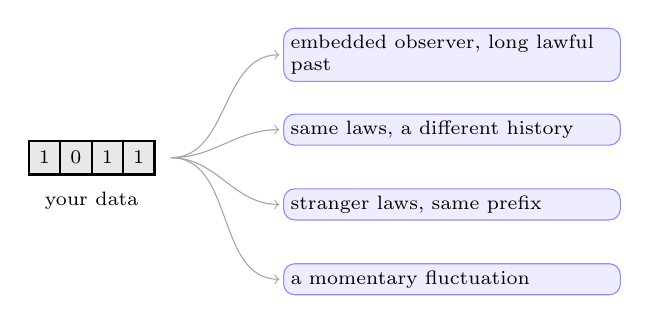
\begin{tikzpicture}[scale=0.95]
  % data prefix (left)
  \foreach \i/\b in {0/1, 1/0, 2/1, 3/1} {
    \draw[thick, fill=gray!18] (\i*0.42,0.9) rectangle (\i*0.42+0.42,1.35);
    \node[font=\scriptsize] at (\i*0.42+0.21,1.125) {\b};
  }
  \node[font=\scriptsize, anchor=north] at (0.84,0.8) {your data};
  % candidate worlds (right)
  \foreach \y/\lbl in {2.5/{embedded observer, long lawful past}, 1.5/{same laws, a different history}, 0.5/{stranger laws, same prefix}, -0.5/{a momentary fluctuation}} {
    \node[font=\scriptsize, anchor=west, draw=blue!45, rounded corners, inner sep=2.5pt, fill=blue!7, text width=4.1cm] at (3.4,\y) {\lbl};
    \draw[->, gray!70] (1.9,1.125) to[out=0,in=180] (3.35,\y);
  }
\end{tikzpicture}
\caption{Two underdeterminations. A finite stretch of data (left) is compatible with many candidate programs (right), and $M$ gives a posterior over those programs. If several observer occurrences match the same data, $M$ alone does not distribute probability among them. ``Which program predicts next?'' and ``which occurrence am I?'' are different questions.}
\label{fig:where-am-i}
\end{figure}

This is where the missing occurrence measure of Chapter 7 would have to do its work, and the literature offers rules to supply it: the Self-Sampling Assumption, which says to reason as if you were a random sample from a chosen reference class; the Self-Indication Assumption, which treats your existence as evidence for hypotheses with more observers like you; and xerographic distributions, which assign first-person weights directly. They disagree about cases such as Sleeping Beauty, the doomsday argument, and Boltzmann observers. None is forced, and each must first say what counts as an occurrence, which is to say where to cut. Appendix~\ref{app:anthropics} surveys them.

The book does not commit to an indexical assumption. So \emph{where am I?}, understood as self-location among occurrences, does not merely have a broad posterior here; it is undefined until extra structure is supplied. That is a limit of the framework, kept visible rather than hidden inside $M$.

\section*{No description contains its center}

Here is why the gap cannot be closed by looking harder. Imagine two beings who between them know every fact there is about their world. One lives on the highest mountain and throws down manna; the other lives on the coldest mountain and throws down thunderbolts. Each knows that both of these things are so. Each knows every proposition that is true of that world, in complete detail, and still neither can say which of the two it is. Nothing in the complete description settles it, because the description contains both of them, and \emph{this one} is not among its sentences.

That is the shape of the gap, and the Library did not make it. A description of the whole, however complete, does not say which part of it is the one reading the description. It can contain every occurrence of you, each with your memories and each thinking \emph{I am here}, and still not contain the fact of which one is this. Nor which later one is next. Those facts are not missing from the description by oversight. They are not the kind of thing a description contains. Philosophers call a world with a \emph{you are here} mark in it a centered world; the mark is the one thing the catalogue of Chapter 2 could not carry. Put it in one sentence, because the rest of the book will use it by name: \emph{no description contains its center}.

The gap has two faces. \emph{Now:} among the occurrences that match your evidence, which one is you? That is the self-location question, and the missing occurrence measure is that question in the Library's currency. \emph{Next:} among the later occurrences, which ones continue you? That is the question of identity over time, and Part III lives in it. Every argument in the family these questions belong to needs three things: a supply of occurrences, a rule for \emph{now}, and a rule for \emph{next}. The rules are cuts.

The supply can come from anywhere. Everett's reading is the supplier with the most physics behind it, and Chapter 8 kept it as the landmark for that reason. But it is not needed. Ordinary cosmology allows a universe that is infinite in space, and in an infinite universe with enough variety every finite arrangement of matter occurs somewhere, and occurs again: on that assumption there are exact duplicates of you, far beyond any horizon, including ones who share your history up to this sentence. Take the thought one step further, as anyone will who has heard the quantum version. Some of those duplicates share your history up to a death and then, by some accident, survive it. So the whole argument that circulates under the name quantum immortality can be run with no quantum mechanics at all: you die here; somewhere, after eons, a pattern with your history up to that moment continues; and for you, the thought goes, the eons were nothing, an instantaneous blip. Eternal inflation supplies the same copies by another route, thermal fluctuation by another, a simulation by another, and the Library read ontically by the broadest route of all. The supplier changes; the argument does not. Its force was never in the physics. It is in the two rules.

Look at what the rules are doing, with the infinite cosmos as the case. The survivor exists whether or not you die. It is there now, in some far region, while you are alive; your death does not bring it into being and sends nothing to it. So \emph{you die, and then you continue as the survivor} is not something the cosmology says. It is the rule for \emph{next} talking. And the same rule, applied evenly, makes the survivor as much you before your death as after, along with every other match, including the ones whose next moment is dissolution. The story of waking up elsewhere picks out the continuations you would prefer and calls the picking a fact. The blip is the same move again. No time passed \emph{for you} between death and the next instance only if there is a you that spans the gap, and that is what is in question. No one experiences the gap, and no one experiences its absence. Even the order of the two events is a convention, since nothing connects the regions; \textit{Worldlines} said why. And the measure gets worse without the quantum, not better. Everett at least offers the Born weights, whatever they are weights of. In an infinite cosmos the ratio of survivor-copies to the rest is infinity over infinity, and every way of regularizing it, cosmologists have found, gives an answer that depends on the cutoff you chose. \emph{Which one is you} has no answer here, not because of anything quantum, but because counting occurrences in an infinite reality needs a measure that nobody has.

There is a tempting way out, and it is the slip of Chapter 6 made one level down. Each supplier comes with a weighting of its own: Born weights on branches, $M$ on programs, nothing at all for infinite space. Read the native weighting as the chance that you are this occurrence, and the gap seems filled. The most principled version of the move uses the book's own prior: weight an occurrence by the length of the shortest program that generates its world \emph{and locates it inside}. That proposal has a name, UDASSA, and Appendix~\ref{app:anthropics} describes it while Appendix~\ref{app:objections} gives it the hearing it deserves. Here, one sentence. The locating program is an index, its length is relative to a machine, and the decision to weight by that length is the choice of a rule. It is a cut, and a good one, for a job. It is not the center found.

So two claims have been hiding in the phrase \emph{the missing occurrence measure}, and they should be kept apart. That the construction supplies none is a finding: $M$ is defined on prefixes, because weights come after cuts, and no carving of occurrences has been supplied. That the book adopts none of the rules on offer is a refusal, of exactly the kind the postulate makes.

And now the sentence this chapter is named for can be said with its status attached. No description contains its center: that much is a finding, and it needs no postulate. Whether there is nonetheless a hidden fact of which occurrence is you, in no description but real, is a question nothing inside could settle either way, exactly like the joints. The book declines to posit one. It reads the center as a cut, the line you draw around \emph{this one}, and that is the postulate applied to you. A refusal, not a finding; and the book says which it is.

\section*{No view from the top}

One hope remains, and it is the one a reader keeps in reserve: even if \emph{I} cannot say where I am, surely someone could. Push the question one more time. Perhaps the failure is only yours, a limitation of being small. Is there anyone for whom the question is settled? A vast intelligence, a simulator running our world, a mind that surveys the whole Library at once and reads off every index and every system without ambiguity? If that overview is occupied by someone, then at least the fact of the matter exists, even where you cannot reach it.

The hope fails in two places, and they are different kinds of failure. The first is a finding, and it needs no postulate. Suppose the overview is occupied; grant the vast mind its survey of everything. The survey is a description, and no description contains its center. The mind can see every occurrence that matches you. It cannot read off which of them is you, because that is not in what it sees, however much it sees. Its survey is larger than yours. It is no closer to a center.

The second is the postulate, and the book says so. The vast mind's survey carves the Library into index and system and self, and the reader's hope was that its carving, at least, is the true one. Here the book declines, as it declined in Chapter 6. Any survey of the Library, however vast the mind that performs it, is a carving, and the book reads none as the structure's own. It cannot show that the mind's carving is not the true one; by Chapter 2's one-way certificate, nothing inside could certify that, in either direction. What it can say is that nothing marks the carving as true, and that it will not crown it. And the hidden fact the reader hoped for, the one about your index, unreachable but at least existing: the book does not deny it. It declines it, for the same reason, and says that nothing could certify it either.

Computability adds a narrower point, not a second proof: no computable procedure can decide, for every program, whether it halts. That limits what any computable mind can know about the Library; it does not by itself rule out a greatest mind, and the argument above does not need it.

Greater intelligence can enlarge a view, correct errors, and discover regularities. It cannot turn its decomposition into the structure's uniquely privileged decomposition, and it cannot find a center in a survey. Power is not privilege. A simulator, if one exists, would know more about the simulated system while still bringing its own representation and boundaries.

Hold onto this; Part III will need it. The book has not disproved every possible greater mind, and the one-way certificate says it could not: a mind that showed itself would be its own proof, and nothing proves an absence. What the book has declined is that any mind's description comes stamped as the view from nowhere, and what it has shown is that no view, from anywhere, contains you as its center. Whatever warmth we can responsibly speak of is encountered and made among observers, not inferred from an imagined overview.

\section*{What the framework permits}

The outside view, combined with a supplier of occurrences and the rules this chapter named, none of which the book adopts, permits descriptions that are uncomfortable to sit with. A small sample, each with what it needs.

\emph{Boltzmann brains.} In some long-lived cosmological models, and under some ways of counting observer occurrences, transient fluctuations can outnumber ordinary observers. If you treated yourself as a random draw from that class, your apparent past could be misleading (Figure~\ref{fig:boltzmann-brain}). It needs a supplier and a rule for \emph{now}.\footnote{Schmidhuber's \emph{speed prior} penalizes computation time and is sometimes discussed near this problem. It is a prior over program outputs, not by itself a probability distribution over observer occurrences, and it does not resolve the reference-class question.}

\begin{figure}[h]
\centering
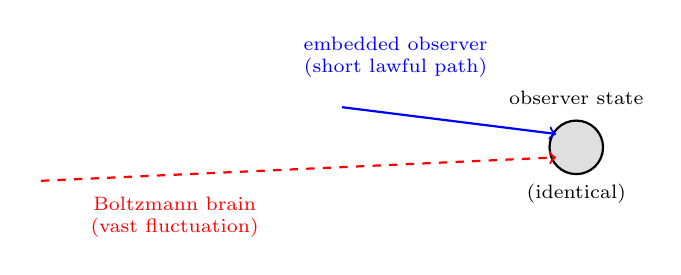
\begin{tikzpicture}[scale=0.85]
  % Common observer state on the right
  \draw[thick, fill=gray!25] (8, 0.8) circle (0.4);
  \node[font=\scriptsize, anchor=south] at (8, 1.3) {observer state};
  \node[font=\scriptsize, anchor=north] at (8, 0.4) {(identical)};

  % Embedded path: short blue arrow from the left
  \draw[thick, blue, ->] (4.5, 1.4) -- (7.7, 1.0);
  \node[font=\scriptsize, anchor=south, blue, text width=3.2cm, align=center] at (5.3, 1.7) {embedded observer (short lawful path)};

  % BB path: very long red dashed arrow from far left
  \draw[thick, red, dashed, ->] (0, 0.3) -- (7.7, 0.65);
  \node[font=\scriptsize, anchor=north, red, text width=3.5cm, align=center] at (2, 0.2) {Boltzmann brain (vast fluctuation)};
\end{tikzpicture}
\caption{Two hypotheses for matching data. A lawful history and a fluctuation could, in principle, contain the same instantaneous observer-state. Comparing their first-person probabilities requires a cosmology and an occurrence measure that this framework does not provide.}
\label{fig:boltzmann-brain}
\end{figure}

\emph{Hellscapes.} Programs can describe worlds of sustained suffering, and nothing in the Library forbids the description. On the outside view such descriptions can be read ontically; on the inside view they need not be. It needs the outside view read ontically, and nothing more. Program weights are not moral weights.

\emph{Dark continuation.} A supplier, plus a rule for \emph{next} and a rule for \emph{now} that spreads first-person weight only over the moments that can report, can generate stories in which experience follows surviving but progressively damaged occurrences. The quantum is dispensable here too. The book names the possibility because careless presentations of the idea called quantum immortality (Chapter 11 takes it up) often omit its darkest implication.

\emph{Versions of you, and of everyone you love.} The outside view permits descriptions in which a matching pattern acts or suffers differently. Calling those patterns versions of a person, asserting that they exist, and assigning weight among them are three additional choices.

One thing should be said plainly here, because this is the sharpest the book has yet been. Describing a possibility does not place you in it, and the framework has supplied no occurrence measure that says otherwise. If this section is destabilizing, step away from it and return to the room, person, or task within reach. ``No cut is privileged'' is a claim about descriptions and boundaries, not a claim that your present experience or personhood is unreal. The framework survives being held at arm's length.

What the book offers in response is not a formal move. It is the chosen response of Part III. The mathematics is silent on what to do; care is what we provide; the rest of the book is what that looks like.

\section*{Where this leaves you}

The coldest part of the picture is now in view. You have met the book's one interpretive commitment:

\begin{quote}
\textbf{The postulate: no cut is privileged.} The book treats no decomposition of the describable totality as view-independently correct. Every carving into worlds, systems, and selves it reads as a cut an observer makes, and none as the structure's own.
\end{quote}

\noindent The book takes it. You may refuse it, as Chapter 7 set out, and keep the mathematics. Everything this chapter catalogued, read as more than a description, needs the optional additions as well.

The book will not engineer answers to questions the framework leaves open, and several stay open: which occurrence is you, which picture is real, whether anything answers to the darkest descriptions. Precision does not remove the darkness; it prevents the book from claiming more darkness than its premises earn.

There is a name for what all of this amounts to, and the next chapter says it.
